% !TEX root = ../VPJ.tex

\chapter{Implementierung}
\label{sec:Implementierung}

Implementierung

\section{Programmstruktur}

\inlinetodo{Was ist noch in Fertigungsplanung}


\begin{figure}[htb]
    \centering
    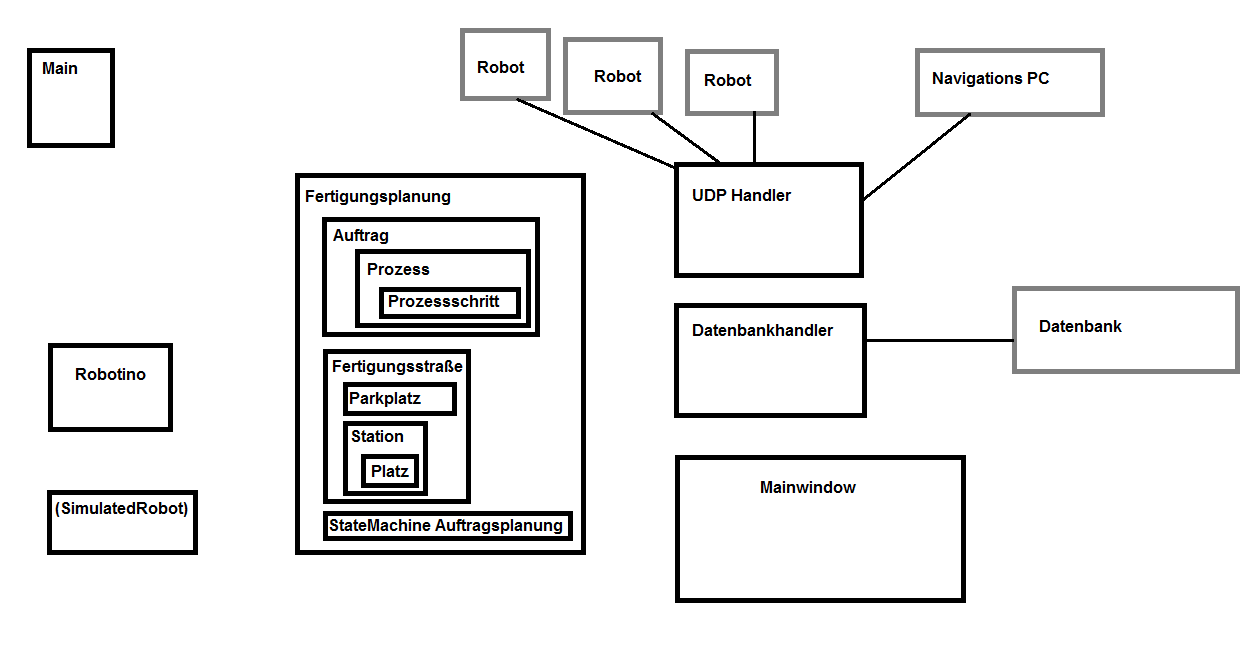
\includegraphics[width=0.9\textwidth]{Abbildungen/Klassendiagramm.PNG}
    \caption{Klassendiagramm}		
    \label{fig:Klassendiagramm}
\end{figure}



\section{Databasehandler}
\section{UDP-Handler} 
\section{Robotino} 

\section{Auftrag, Prozess, Prozessschritt} 
\label{sec:AuftragProzessSchritt}
\subsection{Auftrag}
\label{sec:Auftrag}
\subsection{Prozess}
\label{sec:Prozess}
\subsection{Prozessschritt}
\label{sec:Prozessschritt}


\section{Fertigungsplanung}

\inlinetodo{Was ist noch in Fertigungsplanung}
\inlinetodo{Robotgreifer Changed}
\inlinetodo{RobotStatus Changed}
\inlinetodo{RobotError}
\inlinetodo{Auftrag / Prozess hinzufügen (initialisieren)}
\inlinetodo{HardCode Area}

\subsection{Zustandsdiagramm}

Das Zustandsdiagramm in Abbildung \ref{fig:Auftragsplanung} beschreibt die Logik der Auftragsvergabe an die Roboter. Das Diagramm wurde anschließend als State Machine (vgl. \ref{sec:StateMachines}) implementiert. 

\begin{figure}[htb]
    \centering
    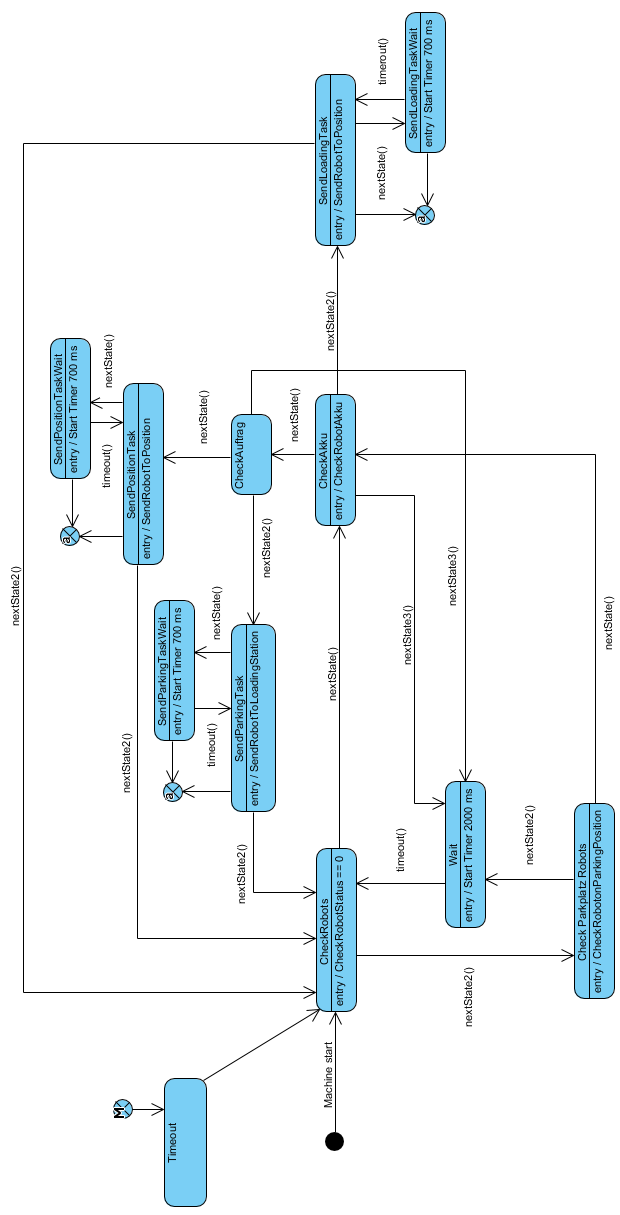
\includegraphics[width=0.8\textwidth]{Abbildungen/Auftragsplanung_rotated.PNG}
    \caption{Zustandsdiagramm der Auftragsplanung}		
    \label{fig:Auftragsplanung}
\end{figure}

In der Abbildung sind die Zustände mit Namen dargestellt. Alle Zustände haben eine komplementäre Funktion, die nach einem Zustandswechsel als Entry-Action aufgerufen wird. Eine genaue Funktionsbeschreibung der Zustände ist in Kapitel \ref{sec:StateMachineImplementierung} zu finden. Um zwischen den Zuständen zu wechseln werden die mit Pfeilen eingezeichneten Transitionen verwendet. Die Pfeilbeschriftung beinhaltet dabei das Signal, welches für den Zustandswechsel genutzt wird. Um das Diagramm übersichtlich zu gestalten, wurden die Timeout-Transitionen nicht vollständig eingezeichnet, sondern enden in einem kreisförmigen Xa-Zustand. Dieser führt direkt zu dem XM-Zustand oben links und leitet in den Zustand Timeout weiter. 

\subsection{State Machine Implementierung}
\label{sec:StateMachineImplementierung}

Im Quellcode werden zunächst alle Zustände erzeugt und der State Machine hinzugefügt. Anschließend werden alle Transitionen zwischen den Zuständen erzeugt und der State Machine hinzugefügt. Hierbei werden definierte Signale genutzt, die zuvor in der Header Datei deklariert wurden. In der Main-Funktion werden abschließend die Zustände mit den entsprechenden zugehörigen Funktionen verknüpft (vgl. \ref{sec:Main}). 

Um die State Machine zu starten wird, nachdem der Initialzustand bekannt gemacht wurde, die Start-Funktion aufgerufen. Eine verkürzte Darstellung der Aufrufe ist in Listing \ref{lst:StartStateMachine} abgebildet. 

\begin{lstlisting}[frame=single, breaklines=true, numbers=left, stepnumber=2, firstnumber=1, numberstyle = \tiny, caption=Start und Initialisierung der State Machine,label=lst:StartStateMachine]
    QStateMachine StateMachine;
    QState *StateCheckRobots = new QState;

    StateMachine.addState(StateCheckRobots);
    StateCheckRobots->addTransition(this, SIGNAL(nextState()), StateCheckAkku);

    StateMachine.setInitialState(StateCheckRobots);
    StateMachine.start();

    QObject::connect(StateCheckRobots, &QState::entered, this, &Fertigungsplanung::CheckRobots);
\end{lstlisting}

\subsubsection{Zustand CheckRobots}

Im Initialzustand der State Machine, CheckRobots, werden alle vier Roboter nacheinander auf Bereitschaft überprüft. Die Reihenfolge der zu überprüfenden Roboter wird dabei durch einen hierfür entwickelten Shuffle-Algorithmus (\ref{sec:shuffle}) bestimmt. 

Ein Roboter gilt als bereit, wenn er als Status 0 zurückgibt, nicht als defekt markiert ist und als lebend gilt. Sobald ein geprüfter Roboter alle drei Kriterien erfüllt wird dieser ausgewählt und in den weiteren Zuständen, gefolgt von CheckAkku, genutzt. Die anderen Roboter werden bis zum nächsten Aufruf des Zustands CheckRobots vernachlässigt.

Sollte keiner der vier Roboter alle drei Kriterien erfüllen wird in den Zustand CheckParkplatzRobots gewechselt.

\subsubsection{Zustand CheckParkplatzRobots}

Wie im Zustand CheckRobots werden alle vier Roboter anhand von Kriterien auf Bereitschaft überprüft. Dazu wird ebenfalls die Reihenfolge zufällig bestimmt.

Anstatt den Roboterstatus wie beim Zustand CheckRobots auf 0 zu prüfen, wird ein Status zwischen 201 und 204 erwartet. Diese vier Stati repräsentieren die vier Parkplätze auf denen sich ein Roboter befinden kann. 

Durch die Aufteilung der Zustände CheckRobots und CheckParkplatzRobots erfolgt eine Priorisierung der Roboter, die sich bereits in den Stationen befinden und einen Auftrag fertig abgearbeitet haben. Nur wenn kein Roboter in den Stationen verfügbar ist wird auf die auf den Parkplatz befindlichen Roboter zurückgegriffen. Dadurch werden Situationen vermindert, in denen sich die Roboter bei der Stationsarbeit gegenseitig behindern.

Sollte keiner der auf den Parkplatz befindlichen Roboter alle weiteren Kriterien erfüllen wird in den Zustand Wait gewechselt.

\subsubsection{Zustand Wait}

Da in Qt aufgrund der eventbasierten Programmierung (vgl. \ref{sec:Eventbasiert}) keine Endlosschleifen vorgesehen sind wurde im Zustand "`Wait"' mittels Timer die Zustandsmaschine künstlich verlangsamt. Ein Entfernen des Zustands führt zum Programmabsturz, da in kürzester Zeit die interne Eventliste voll geschrieben wird. Auf externe Events wie Mauseingaben oder Ereignisse vom Betriebssystem könnte somit nicht mehr reagiert werden. 

Durch den Zustand Wait können andere Programmevents und Ereignisse des Betriebssystems abgearbeitet werden, während 2000 ms auf das timeout()-Signal des Timers gewartet wird. 

Nach Ablauf des Timers wird in den Initialzustand CheckRobots gewechselt.

\subsubsection{Zustand CheckAkku}

Der Zustand CheckAkku gewährleistet einen Tiefentenladungsschutz der Roboter. Sobald ein Roboter in den ersten beiden Zuständen ausgewählt wurde wird überprüft, ob sein Akkustand größer gleich 25 Prozent ist. Es wird davon ausgegangen, dass kein Auftrag plus eine Fahrt zum Laden mehr als 25 Prozent Akku verbraucht. Der Wert wurde empirisch ermittelt. 

Sollte der Akkustand unter 25 Prozent liegen, wird der Roboter über Zustand SendLoadingTask zu einer freien Ladestation geschickt. Wenn keine Ladestation frei ist wird in den Zustand Wait gewechselt. 
Bei einem Akkustand von über 25 Prozent wird der Zustand CheckAuftrag aufgerufen. 

\subsubsection{Zustände SendLoadingTask, SendParkingTask, SendPositionTask}

Um bei Kommunikation mit den Robotern in den Zuständen SendLoadingTask, SendPositionTask und SendParkingTask sicherzustellen, dass die Nachricht empfangen wurde, wird diese mehrfach gesendet, bis die Übertragung erfolgreich war (siehe Kapitel \ref{sec:sequenzdiagram}). Es wird nach jedem Sendevorgang ein kurzer Wartezustand aufgerufen, der, gleich dem Zustand Wait, einen Programmabsturz verhindert. Mit dem individuellen Wartezustand kann ebenfalls das bei aktuell 700 ms angesetzte Sendeintervall eingestellt werden. 

Aus allen den drei Send......Task Zuständen und ihren zugehörigen Wartezuständen kann über ein Ablauf eines Timers in den Zustand Timeout gewechselt werden. Der Timer wird beim erstmaligen Eintritt in einen der Zustände Send......Task gestartet und läuft nach 25 Sekunden ab. Dieser Timer gewährt eine Absturzsicherheit des Programms bei Roboterausfall oder anderweitigem Fehlschlagen der Kommunikation. 

In allen drei Send.....Task Zuständen wird ein erfolgreicher Sendevorgang damit erkannt, dass der Roboterstatus nicht mehr 0 ist, und der Roboter sich nicht mehr auf einem Parkplatz befindet. Solange die beiden Bedingungen nicht erfüllt sind wird weiter an den Roboter gesendet. 

Wenn im Zustand SendLoadingTask die Nachricht erfolgreich versendet wurde, wird der Timer für das Timeout gestoppt, und die benötigte Ladestation in der Visualisierung und in der Datenbank reserviert. Abschließend wird in den Initialzustand gewechselt.

Der Zustand SendParkingTask verhält sich Analog dem SendLoadingTask, nur wird bei erfolgreicher Nachrichtenversendung der benötigte Parkplatz reserviert.

Bei dem Zustand SendPositionTask, in dem ein Auftrag aus der Planung an den Roboter verschickt wurde, werden nach erfolgreichem Nachrichtenversand mehrere Aktionen durchgeführt. Zunächst wird der Timeout-Timer gestoppt. Sollte der Auftrag den ersten Prozessschritt, also das Abholen eines Werkstücks im Lager an Station 1, beinhalten wird der Schreibkopf des RFID neu beschrieben. In der Datenbank wird außerdem dem Start- und Zielarbeitsplatz der genutzte Roboter zugeordnet. Am Startarbeitsplatz wird das vorhandene Werkstück in der Datenbank entfernt und dem Zielarbeitsplatz zugeordnet. Die beiden Stationen werden außerdem Reserviert um zu verhindern, dass ein anderer Roboter an die zu bearbeitenden Stationen geschickt wird. Somit ist eine erste Kollisionsvermeidung implementiert. Zuletzt wird in der Datenbank das genutzte Werkstück dem Roboter zugewiesen. Auch in der Visualisierung werden Start- und Zielarbeitsplatz reserviert. Schlussendlich wird in der Visualisierung der Tooltip (vgl. Kapitel \ref{sec:tooltips}) des Start- und Zielarbeitsplatz aktualisiert.

\subsubsection{Zustand CheckAuftrag}

Der Zustand CheckAuftrag enthält die Vergabe der Aufträge an die Roboter. 
Dazu wird zunächst in der Auftragsliste jeder Auftrag auf unfertige Prozesse untersucht und diese folgend an eine neu erzeugte Prozessliste angehängt (vgl. Abschnitt \ref{sec:AuftragProzessSchritt}). Jeder Prozess der so erzeugten Prozessliste wird anschließend auf die Möglichkeit der Bearbeitung geprüft. Sofern eine der folgenden Prüfungen fehlschlägt wird der nächste Prozess geprüft.

Dazu wird zunächst überprüft ob sich der Prozess schon in Bearbeitung befindet. 

Es wird geprüft ob die Start und Zielstation nicht durch einen Roboter reserviert ist.

Sollte der nächste Prozessschritt der bearbeitet werden muss an der Lagerstation (Station 1) sein, so wird gewährleistet, dass sich ein Werkstück im Lager befindet und dieses ausgewählt. 

Es wird geprüft ob eine der beiden Zielarbeitsplätze der Zielstation frei ist, also weder reserviert noch defekt und anschließend ausgewählt. 

Wenn alle Vorbedingungen für einen der Prozesse eintreffen wird der Zustand direkt verlassen und der Auftrag wird an den ausgewählten Roboter im Zustand SendPositionTask gesendet. 

Sollten alle Prozesse zu keinem Sendevorgang geführt haben, das heißt es ist entweder kein Auftrag vorhanden oder oder das senden wurde blockiert, so wird der aktuell ausgewählte Roboter zum Parken geschickt (Zustand SendParkingTask), sofern er sich noch nicht auf einem Parkplatz befindet. Sonst wird in den Initialzustand gewechselt.

\subsection{Shuffle-Algorithmus}
\label{sec:shuffle}

Der Shuffle-Algorithmus dient dazu, die Roboter in zufälliger Reihenfolge abzuarbeiten, um eventuelle Dead-Locks zu vermeiden. Ein solcher Dead-Lock könnte zum Beispiel eintreten, wenn Roboter 1 und 2 an der Ladestation sind, Roboter 3 zum laden geschickt werden müsste, jedoch warten muss. Roboter 4 würde dabei, selbst wenn er bereit wäre einen Auftrag abzuarbeiten nie überprüft werden.

Zurückgegeben wird eine Liste in der die Zahlen 1 bis 4 in zufälliger Reihenfolge vorliegen. Der Algorithmus ist optimiert gegenüber der Anzahl an Systemaufrufen für eine Zufallszahl. Andernfalls wäre es einfacher solange eine Zufallszahl zurückgeben zu lassen,  wie die Liste diese noch nicht enthält.

Um die Roboterreihenfolge festzulegen werden vier Schritte durchgeführt. Im ersten Schritt wird eine leere Liste erzeugt und eine zufällige Zahl zwischen 1 und 4 an die erste Stelle geschrieben (Listing \ref{lst:shuffle} Zeile 1-3). 

\begin{lstlisting}[frame=single, breaklines=true, numbers=left, stepnumber=2, firstnumber=1, numberstyle = \tiny, caption=Shuffle-Algorithmus,label=lst:shuffle]
    QList<int> liste;
    int i = QRandomGenerator::global()->bounded(1, 5);
    liste.append(i);
    i = QRandomGenerator::global()->bounded(1, 4);
    (liste.contains(i)) ? liste.append(i+1) : liste.append(i);
    i = QRandomGenerator::global()->bounded(1, 3);
    if (liste.contains(i))
    {
        if (liste.contains(i+1))
        {
            liste.append(i+2);
        }
        else
        {
            liste.append(i+1);
        }
    }
    else
    {
        liste.append(i);
    }

    if (!liste.contains(1)) {liste.append(1);}
    else if (!liste.contains(2)) {liste.append(2);}
    else if (!liste.contains(3)) {liste.append(3);}
    else if (!liste.contains(4)) {liste.append(4);}
    return liste;
\end{lstlisting}

Im zweiten Schritt wird eine Zufallszahl zwischen 1 und 3, wenn sie noch nicht enthalten ist, in die Liste geschrieben oder um eins inkrementiert und in die Liste geschrieben (Listing \ref{lst:shuffle} Zeile 4f). 

Um die nächste Zahl hinzuzufügen wird im dritten Schritt (Listing \ref{lst:shuffle} Zeile 6-21) eine Zufallszahl zwischen 1 und 2 erzeugt und in die Liste geschrieben, sollte sie nicht vorhanden sein. Wenn sie schon existiert wird sie um eins inkrementiert und erneut überprüft ob die inkrementierte Zahl in der Liste ist. Aufgrund der Maximalgröße von 4 kann der Algorithmus so alle Fälle abdecken.
 
Zuletzt wird die noch fehlende Zahl der Liste ergänzt (Listing \ref{lst:shuffle} Zeile 22ff) und die Liste zurückgegeben. 

\section{Mainwindow}

\section{Main}
\label{sec:Main}
\inlinetodo{StateMachine Connections beschreiben / erwähnen - genau eine funktion zu einem State}
\section{Weitere Klassen}


